\documentclass[12pt,a4paper]{article}
\usepackage[utf8]{inputenc} %polskie znaki
\usepackage[T1]{fontenc}	%polskie znaki
\usepackage{amsmath}		%matematyczne znaczki :3
\usepackage{enumerate}		%Dodatkowe opcje do funkcji enumerate
\usepackage{geometry} 		%Ustawianie marginesow
\usepackage{graphicx}		%Grafika
\usepackage{wrapfig}		%Grafika obok textu
\usepackage{float}			%Allows H in fugire
\usepackage{hyperref}		%Allows hyperlinks
%\pagestyle{empty} 			%usuwa nr strony
\usepackage{todonotes}		%Todo notatki
\usepackage{lipsum}         %Lorem text
\usepackage{ntheorem}   	% for theorem-like environments
\usepackage{mdframed}   	% for framing
\usepackage{subcaption}		% subfigure (image placing)
\usepackage{pdfcomment}		% Komentarze (z bazowego pdf'a)
\usepackage{xparse}			% New commands with optional arguments
\usepackage{ifthen}			% If then - funkcje!
\usepackage{expl3}			% Deklarowanie zmiennych

\newgeometry{tmargin=2cm, bmargin=2cm, lmargin=2cm, rmargin=2cm} 

%Counter commands{
	\newcounter{counter} % Creates a new counter
	\setcounter{counter}{1} % Sets the counter to 5
	\newcommand{\counter}[1]{
		\arabic{#1} \stepcounter{#1} 
	}
	\newcommand{\counterreset}[1]{\setcounter{#1}{1}}
	%}

%Define styles{
	\theoremstyle{break}
	\theoreminframepreskip{0.5cm}
	\theoremheaderfont{\bfseries}
	\newmdtheoremenv[%
	linecolor=white,%
	innertopmargin=\topskip,
	shadowsize=0,%
	innertopmargin=5,%
	innerbottommargin=5,%
	leftmargin=10,%
	rightmargin=10,%
	backgroundcolor=gray!20,%
	innertopmargin=0pt,%
	ntheorem]{zad}{Zadanie}
	
	\mdfdefinestyle{zadanie}{
		linecolor=white,%
		innertopmargin=5,%
		innerbottommargin=5,%
		leftmargin=10,%
		rightmargin=10,%
		backgroundcolor=gray!20,%
		innertopmargin=8,
		innerbottommargin=8,
		skipabove = 5,
	}
	\mdfdefinestyle{wzor}{
		linecolor=cyan,%
		linewidth=2pt,%
		innertopmargin=8,
		innerbottommargin=8,
		leftmargin=10,%
		rightmargin=10,%
		backgroundcolor = white, 
		fontcolor = black,
		skipabove = 5,
		skipbelow = 5,
	}
	%}

%Zadania templatex%{
	\newcommand{\Wzor}[1]{
		\begin{mdframed}[style=wzor]
			\centering #1
		\end{mdframed}
	}
	\newcommand{\ZadanieTextowe}[1]{
		\begin{mdframed}[style=zadanie]
			\textbf{Zadanie \counter{counter} } \\
			#1
		\end{mdframed}
	}
	\newcommand{\Zadanie}[2]{
		\ZadanieTextowe{#1}
		#2
	}
	\newcommand{\ZadanieABCD}[6]{
		\ZadanieTextowe{#1}
		#2 \\\\
		\begin{tabular}{p{7cm} p{7cm}}
			\textbf{A. }#3&
			\textbf{B. }#4\\\\
			\textbf{C. }#5&
			\textbf{D. }#6\\
		\end{tabular}
	}
	\newcommand{\ZadanieABCDEF}[8]{
		\ZadanieTextowe{#1}
		#2 \\\\
		\begin{tabular}{p{7cm} p{7cm}}
			\textbf{A. }#3&
			\textbf{B. }#4\\\\
			\textbf{C. }#5&
			\textbf{D. }#6\\\\
			\textbf{E. }#7&
			\textbf{F. }#8\\\\
		\end{tabular}
	}
	\newcommand{\Zadanietwoxtwo}[5]{
		\ZadanieTextowe{#1}
		\begin{tabular}{p{7cm} p{7cm}}
			\textbf{a)} #2&
			\textbf{b)} #3\\\\
			\textbf{c)} #4&
			\textbf{d)} #5\\\\
		\end{tabular}
	}
	\newcommand{\Zadanietwoxthree}[7]{
		\ZadanieTextowe{#1}
		\begin{tabular}{p{7cm} p{7cm}}
			\textbf{a)} #2&
			\textbf{b)} #3\\\\
			\textbf{c)} #4&
			\textbf{d)} #5\\\\
			\textbf{e)} #6&
			\textbf{f)} #7\\\\
		\end{tabular}
	}
	\newcommand{\Zadanietwoxfour}[9]{
		\ZadanieTextowe{#1}
		\begin{tabular}{p{7cm} p{7cm}}
			\textbf{a)} #2&
			\textbf{b)} #3\\\\
			\textbf{c)} #4&
			\textbf{d)} #5\\\\
			\textbf{e)} #6&
			\textbf{f)} #7\\\\
			\textbf{g)} #8&
			\textbf{h)} #9\\\\
		\end{tabular}
	}
	%}

\begin{document}
	\begin{center}
		\LARGE Pojęcie funkcji
	\end{center}
	\ZadanieTextowe{Które z podanych niżej zapisów są, a które nie są funkcjami:}
	\begin{enumerate}[a)]
		\item $f(x)=x^3-2x^2-3x+4$
		\item Każdej osobie przyporządkowujemy jego nazwisko
		\item Każdemu państwu przyporządkowujemy jego stolice
		\item Każdej mamie przyporządkowujemy jej dzieci
		\item 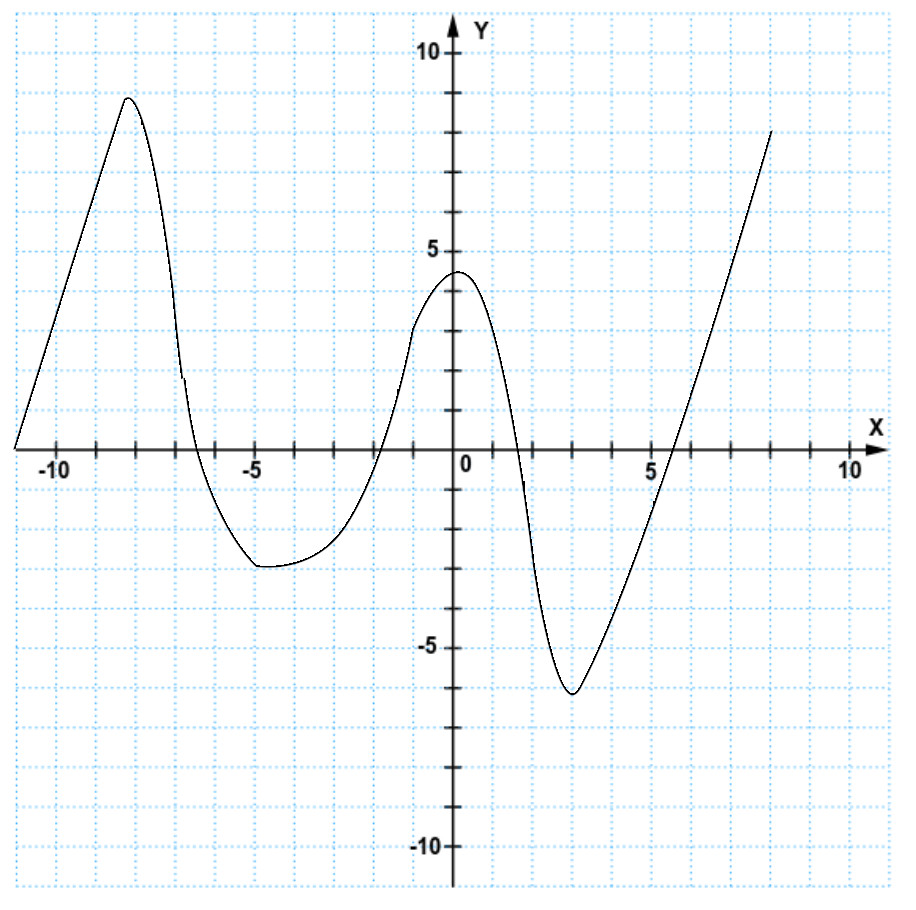
\includegraphics[width=5cm,height=5cm]{z2_1_2.jpg}
		\item 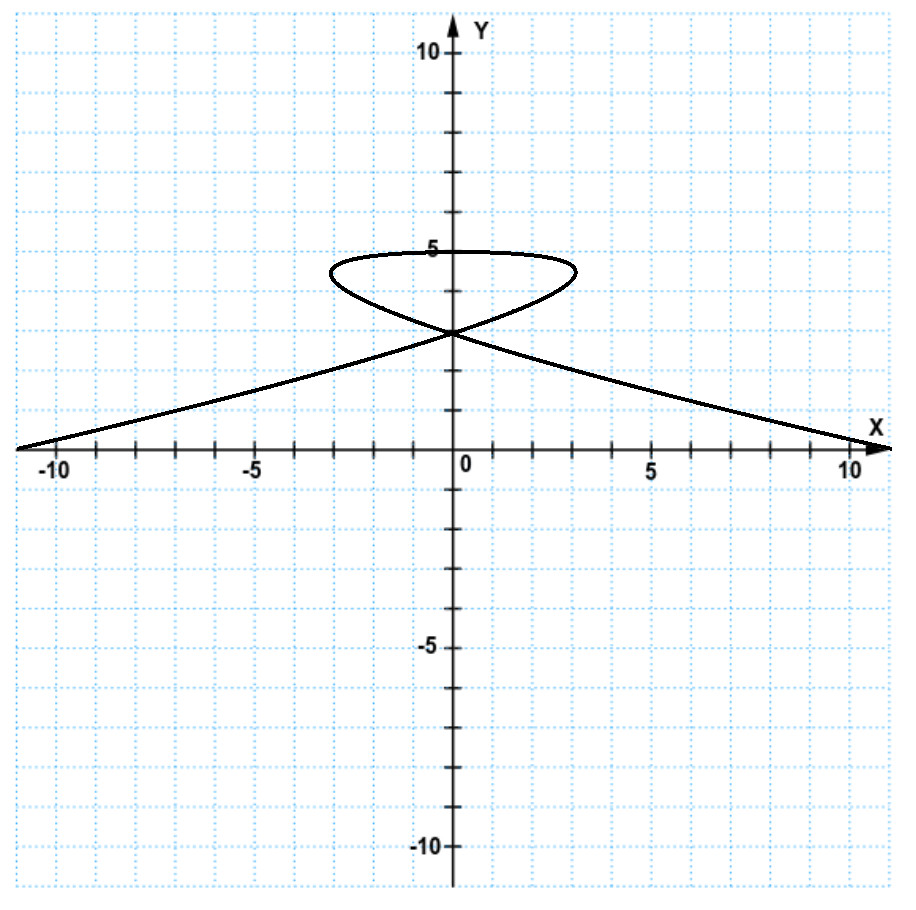
\includegraphics[width=5cm,height=5cm]{z2_1_1.jpg}
		\item Każdemu uczniowi klasy 4C przyporządkowujemy jego ocene ze sprawdzianu
		\item Każdemu samochodowi przyporządkowujemy jego właściciela
		\item Każdej osobie przyporządkowujemy jego auto
	\end{enumerate}

	\newpage

	\Zadanie{Dla poniżych funkcji zapisz ich:}{\begin{enumerate}[a)]
			\item Dziedzinę
			\item Zbiór wartości
			\item Miejsca zerowe
			\item Przedziały monotoniczności
			\item Kiedy funkcja przyjmuje wartości nieodatnie, a kiedy ujemne
			\item Wartość jaką funkcja przyjmuje dla argumetów: -2, 0 i 3
			\item Argumenty dla których funkcja przyjmuje wartość równą 2
	\end{enumerate}}
	\begin{enumerate}[1.]
		\item 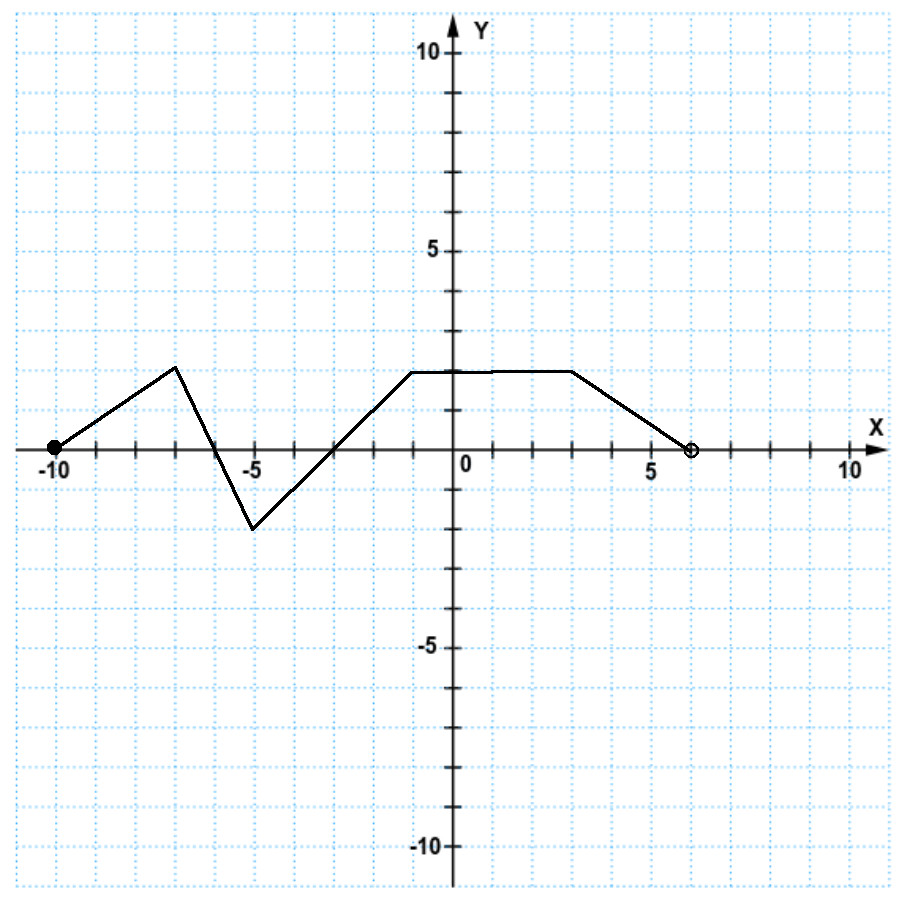
\includegraphics[width=10cm,height=10cm]{z2_2_1.jpg}
		\item 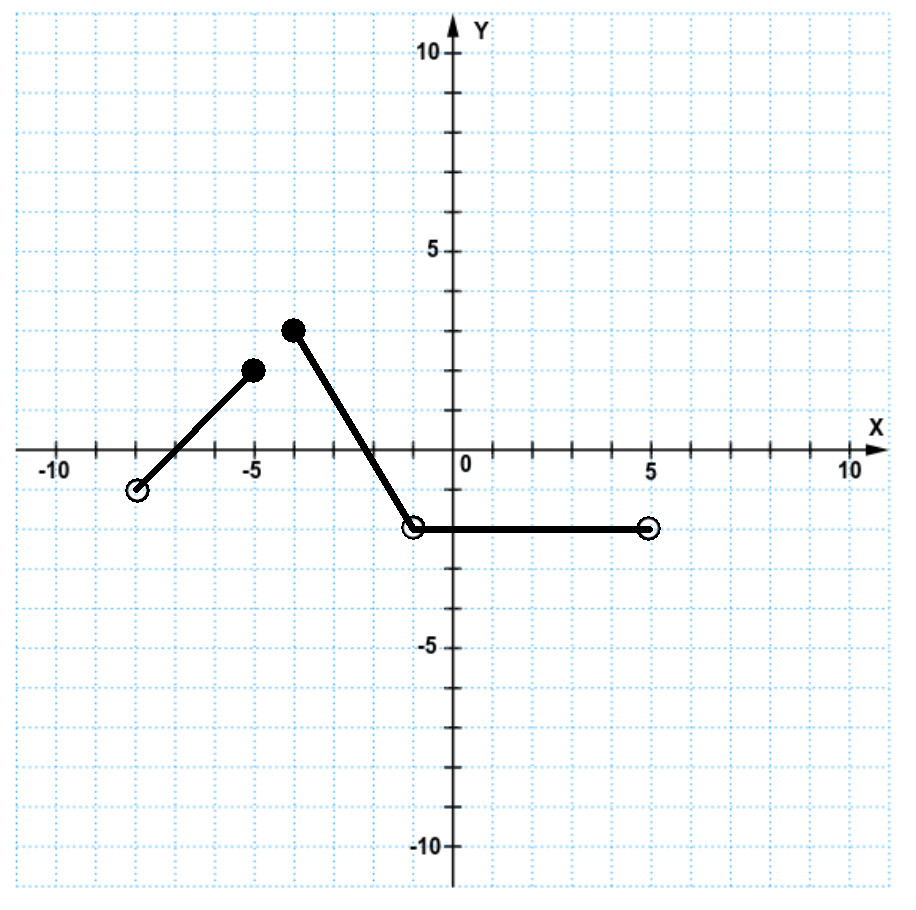
\includegraphics[width=10cm,height=10cm]{z2_2_2.jpg}
		\item 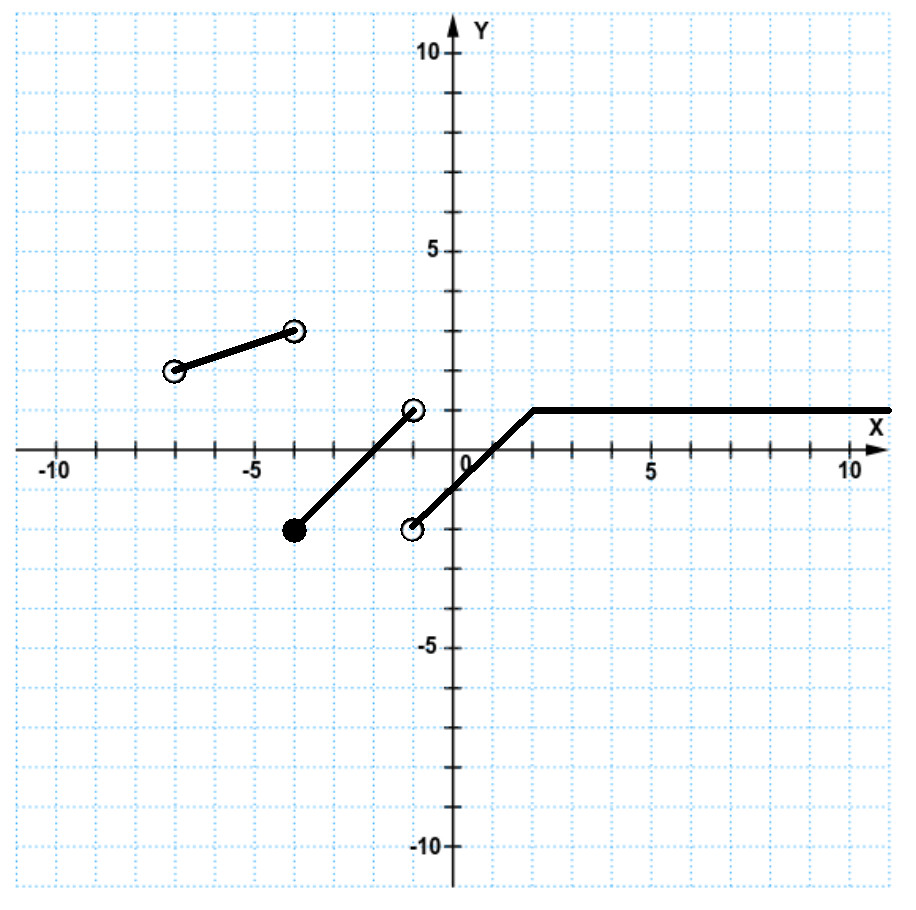
\includegraphics[width=10cm,height=10cm]{z2_2_3.jpg}
		\item 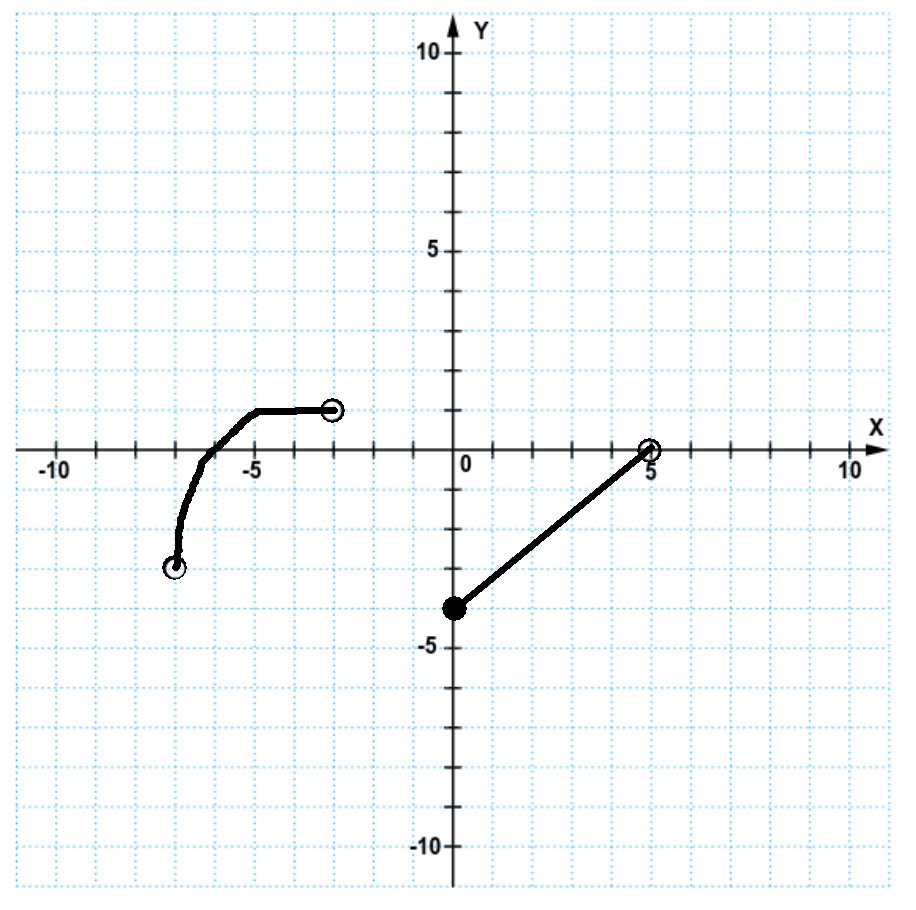
\includegraphics[width=10cm,height=10cm]{z2_2_4.jpg}
		\item 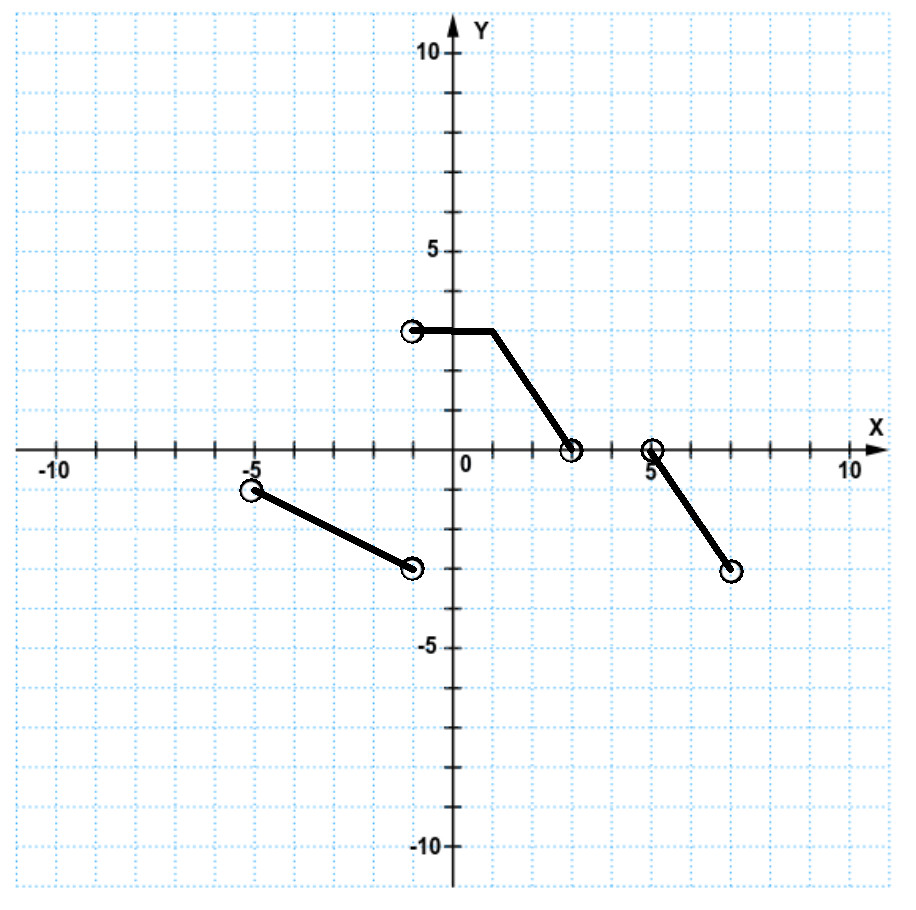
\includegraphics[width=10cm,height=10cm]{z2_2_5.jpg}
		%\item 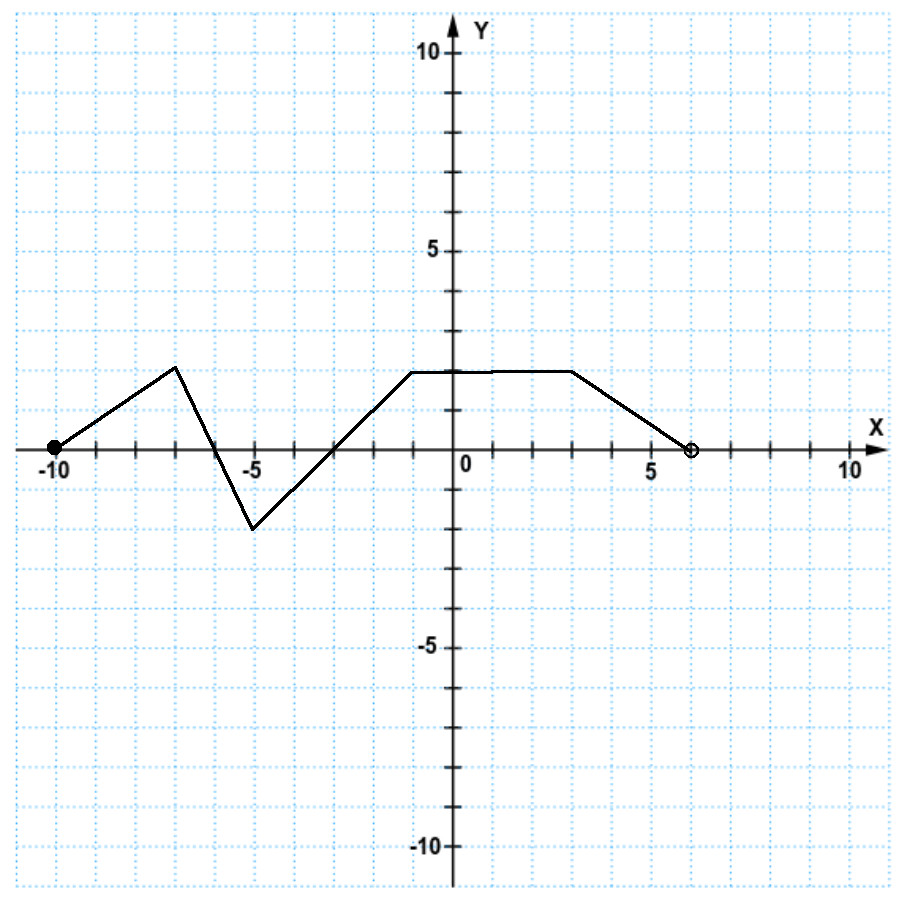
\includegraphics[width=10cm,height=10cm]{z2_2_1.jpg}
	\end{enumerate}
	
	\newpage

	\ZadanieTextowe{Na podstawie wykresów funcji z Zadania 2 narysuj:}
	\begin{enumerate}[a)]
		\item (1.) jako $f(x)$ => $g(x)=f(x-3)-4$
		\item (4.) jako $f(x)$ => $g(x)=f(x+2)+3$
		\item (3.) jako $f(x)$ => $g(x)=f(x+4)-5$
		\item (2.) jako $f(x)$ => $g(x)=-f(x)$
		\item (5.) jako $f(x)$ => $g(x)=-f(x+6)$
		\item (2.) jako $f(x)$ => $g(x)=f(-x)+3$
		\item (4.) jako $f(x)$ => $g(x)=-f(-x)$
		\item (2.) jako $f(x)$ => $g(x)=|f(x)|$
		\item (5.) jako $f(x)$ => $g(x)=-|f(x)|$
		\item (1.) jako $f(x)$ => $g(x)=|f(x)|+4$
		\item (1.) jako $f(x)$ => $g(x)=|f(x)+4|$
		\item (4.) jako $f(x)$ => $g(x)=f(|x|)$
		\item (3.) jako $f(x)$ => $g(x)=f(|x|)-2$
		\item (5.) jako $f(x)$ => $g(x)=f(|x-3|)$
		\item (4.) jako $f(x)$ => $g(x)=f(|x|-3)$
		\item (1.) jako $f(x)$ => $g(x)=f(-|x|)$
		\item (3.) jako $f(x)$ => $g(x)=-|f(|x|)|$
		\item (5.) jako $f(x)$ => $g(x)=|f(-|x|+5)-5|$
	\end{enumerate}
\newpage

\counterreset{counter}
	\begin{center}
		\LARGE Zbiór zadań - pojęcie funkcji
	\end{center}
	\Zadanie{Dla poniżych funkcji zapisz ich:}{\begin{enumerate}[a)]
			\item Dziedzinę
			\item Zbiór wartości
			\item Miejsca zerowe
			\item Przedziały monotoniczności
			\item Kiedy funkcja przyjmuje wartości nieodatnie, a kiedy ujemne
			\item Wartość jaką funkcja przyjmuje dla argumetów: -2, 0 i 3
			\item Argumenty dla których funkcja przyjmuje wartość równą 2
	\end{enumerate}}

	\begin{enumerate}[1.]
		\item 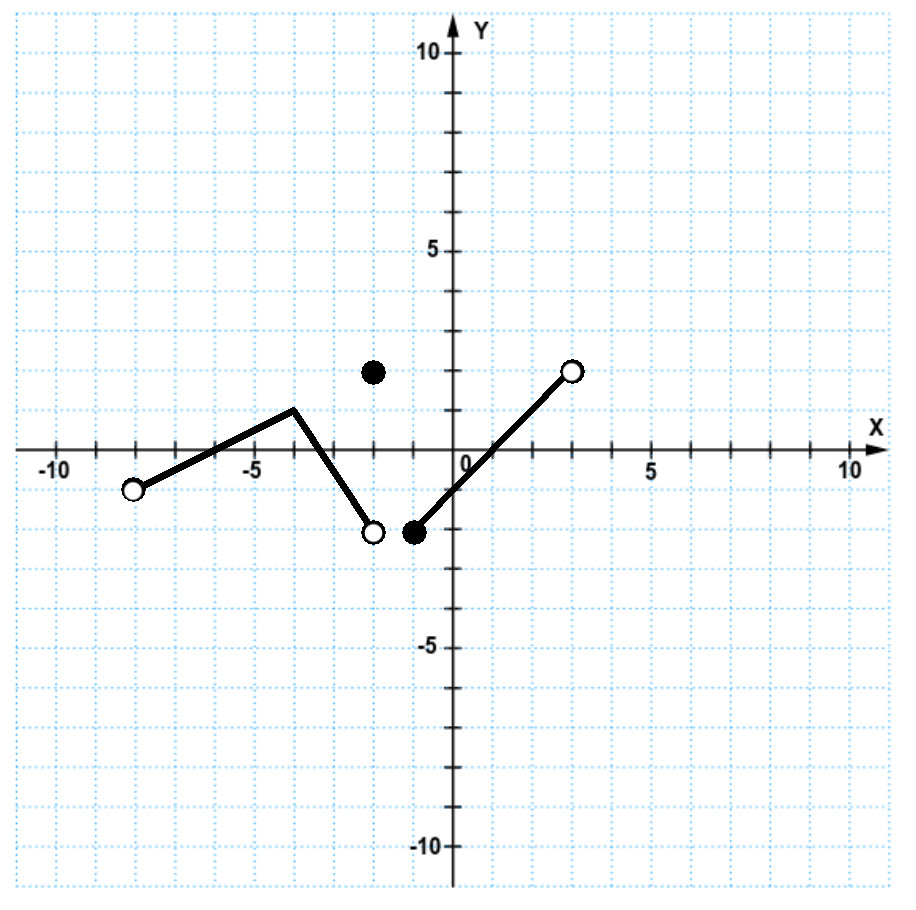
\includegraphics[width=10cm,height=10cm]{z2_3_1.jpg}
		\item 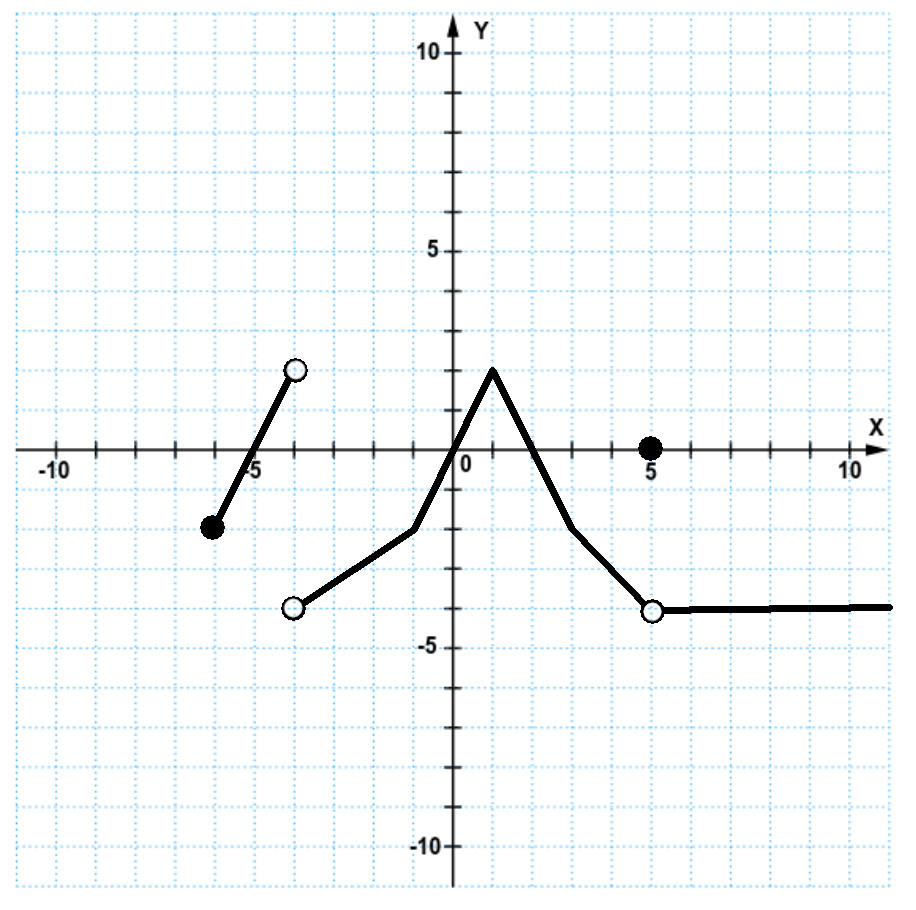
\includegraphics[width=10cm,height=10cm]{z2_3_2.jpg}
		\item 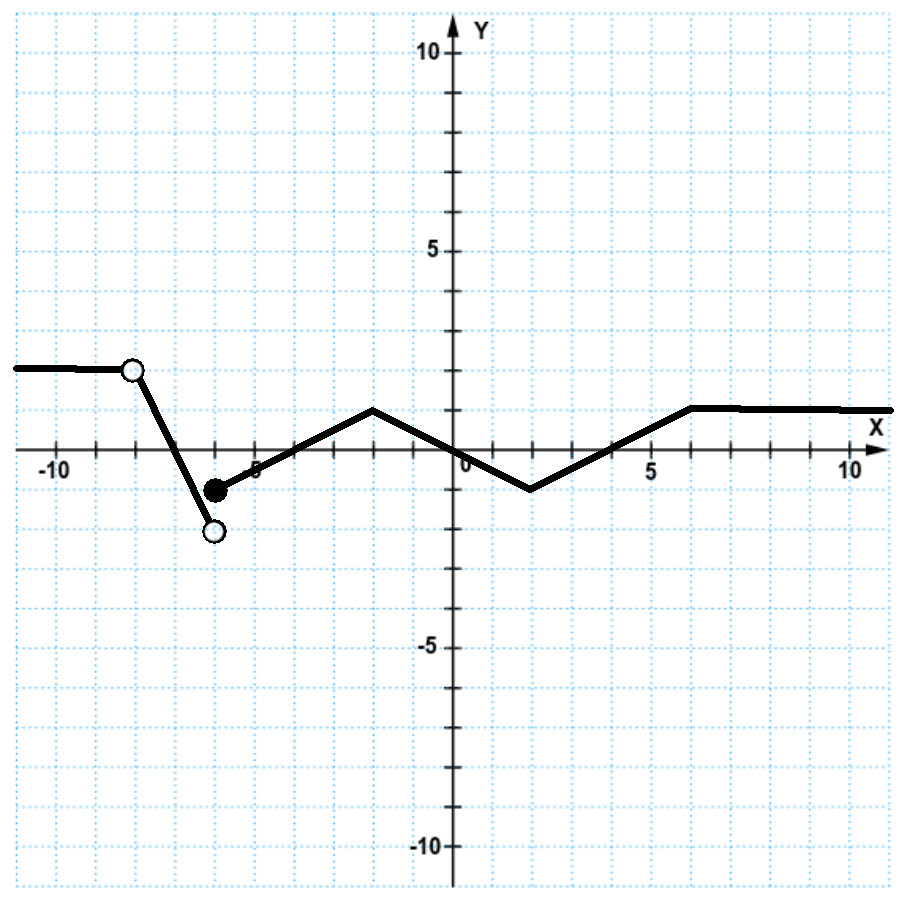
\includegraphics[width=10cm,height=10cm]{z2_3_3.jpg}
	\end{enumerate}

	\newpage
		\ZadanieTextowe{Na podstawie wykresów funcji z Zadania 2 narysuj:}
	\begin{enumerate}[a)]
		\item (1.) jako $f(x)$ => $g(x)=f(x-2)-3$
		\item (2.) jako $f(x)$ => $g(x)=f(x)+3$
		\item (3.) jako $f(x)$ => $g(x)=f(x+1)-5$
		\item (2.) jako $f(x)$ => $g(x)=-f(x)$
		\item (3.) jako $f(x)$ => $g(x)=-f(x)+1$
		\item (2.) jako $f(x)$ => $g(x)=f(-x)+3$
		\item (1.) jako $f(x)$ => $g(x)=-f(-x)$
		\item (2.) jako $f(x)$ => $g(x)=|f(x)|$
		\item (3.) jako $f(x)$ => $g(x)=f(|x|)$
	\end{enumerate}
\end{document}